\documentclass{standalone}
\usepackage{pgfplots}
\pgfplotsset{compat=1.18}

\begin{document}
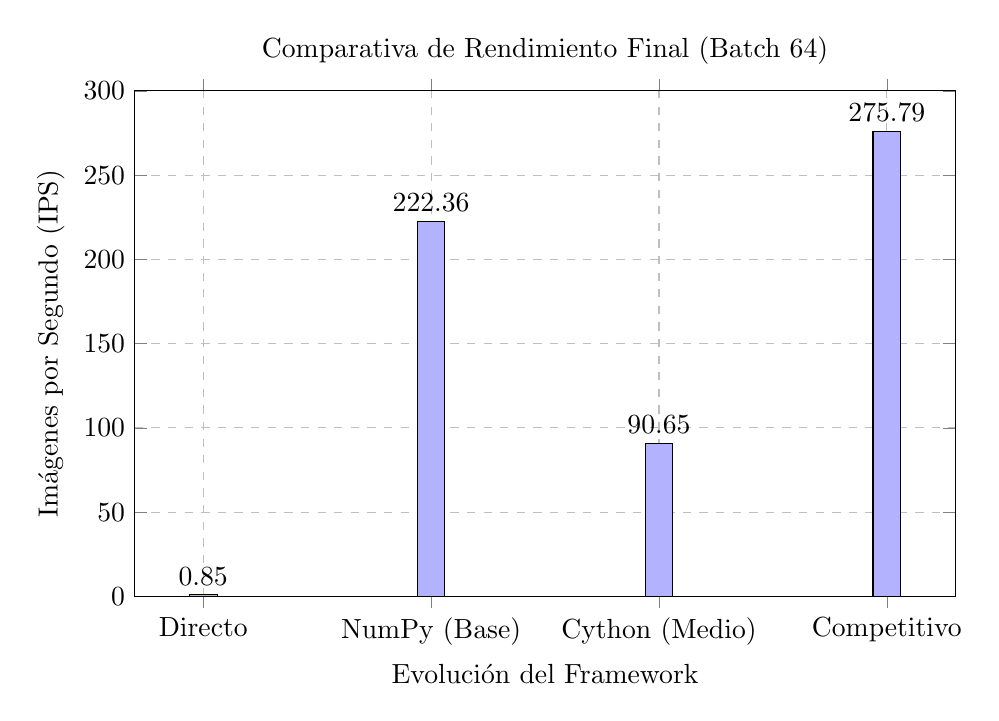
\begin{tikzpicture}
\begin{axis}[
    ybar,
    width=12cm,
    height=8cm,
    ylabel={Imágenes por Segundo (IPS)},
    xlabel={Evolución del Framework},
    symbolic x coords={Directo, NumPy (Base), Cython (Medio), Competitivo},
    xtick=data,
    nodes near coords,
    nodes near coords align={vertical},
    title={Comparativa de Rendimiento Final (Batch 64)},
    grid=both,
    grid style={dashed},
    ymin=0, ymax=300
]
\addplot[fill=blue!30] coordinates {
    (Directo, 0.85)
    (NumPy (Base), 222.36)
    (Cython (Medio), 90.65)
    (Competitivo, 275.79)
};
\end{axis}
\end{tikzpicture}
\end{document}
